\ifdefined\latexbokFontdir\else\def\latexbokFontdir{../../fonts}\fi
\ifdefined\latexbokFiguredir\else\def\latexbokFiguredir{../../examples}\fi
\documentclass[lang=sv,ptsize=10pt,font=none,nomath,titles=bf,../../a4.tex]{subfiles}
\begin{document}
\section{Referenser med \pack{biblatex}}\label{sec:5}
En stor fördel med \LaTeX{} är att man kan automatisera hanteringen av
till exempel referenser. Paketet \pack{biblatex}, tillsammans med
programmet \cli{biber}\footnote{Tekniskt sett kan även
\BibTeX{} användas tillsammans med \pack{biblatex}, men det finns egentligen ingen anledning att göra det. Den som är intresserad av
\BibTeX{}, det gamla systemet för att hantera referenser, hänvisas till introduktionen i \textcite{Fenn06} samt \BibTeX{}-manualen
\parencite{Patashnik88a}.}, gör detta mycket enkelt genom att låta dig
samla alla dina referenser i en extern databas, som man sedan läser in
och hänvisar till. Denna databasen lagras i ett textbaserat format, så
den går att hantera med samma program du skriver \LaTeX-kod i, eller i
ett specialiserat program\footnote{Exempel på sådana är \emph{JabRef},
\emph{BibDesk} och \emph{refbase}.}.

Användningen av \pack{biblatex}-\cli{biber} (där \pack{biblatex} är det
\LaTeX-paket som hanterar typsättningen, och \cli{biber} är ett externt
program som behandlar och sorterar referenserna) kan delas upp i några
olika delar. Till att börja med kommer vi att diskutera formatet av
själva referensdatabasen. Därefter diskuteras paketet \pack{biblatex},
några av dess viktigaste inställningar och stilar, och till sist
sammanfattas användningen av de två tillsammans, speciellt hur man
refererar och genererar referenslistan.

\cite{Lehman13} % biblatex-manual
\cite{Kime13} % biber-manual

\subsection{Referensdatabaser}
Databaserna \pack{biblatex} använder är, som nämndes tidigare, helt
vanliga textfiler. Dessa innehåller ett antal block, ett per referens
i databasen, som i sin tur innehåller fält med information om varje
referens. Ett typiskt block innehåller en nyckel (som används när man
sedan i \LaTeX-dokumentet refererar till referensen), en titel, en
författare och ett årtal. Beroende på vilken typ av referens (bok,
artikel, och så vidare) det handlar om kan även andra fält finnas med.

\begin{kod}[tbp]
	\centering
	\vfil\cprotect[mm]\ifdraft{\inputminted[frame=single]{latex}{\latexbokFiguredir/5/bibdata.bib}}{\inputminted[frame=single,bgcolor=mintedbg,rulecolor=\color{mintedbg}]{latex}{\latexbokFiguredir/5/bibdata.bib}}\vfil
	\caption{En enkel exempelreferens ur en referensdatabas.}
	\label{ex:bibtex}
\end{kod}

\Cref{ex:bibtex} visar ett block ur en referensdatabas. Blocket inleds
med en blocktyp (\texttt{@article}), som indikerar vilken typ referensen
har, och den nyckel som används när man refererar till källan
(\texttt{Hassanpour08}). Därefter följer ett antal självförklarande
fält som lagrar information om referensen, som i det här fallet är en
artikel ur en tidsskrift. En del av dessa fält är obligatoriska (bland
annat titel och författare), medan andra är frivilliga (till exempel
\texttt{month} och \texttt{doi}). \Cref{tab:blocktyper} listar de några
blocktyper och en del av de obligatoriska/frivilliga fält som hör till.
En fullständig förteckning finns i \textcite[7\psqq]{Lehman13}.

\begin{table}[bp]
	\begin{minipage}{0.98\textwidth}
		\newlength{\oldfboxsep}\setlength{\oldfboxsep}{\fboxsep}
		\setlength{\fboxsep}{0pt}
		\renewcommand{\r}{% (fold)
			\setlength{\fboxsep}{\oldfboxsep}%
			\colorbox{required}{\color{required}o}%\checkmark}%
		} % (end)
		\renewcommand{\o}{% (fold)
			\setlength{\fboxsep}{\oldfboxsep}%
			\colorbox{optional}{\color{optional}v}%\Large$\circ$}%
		} % (end)
		\renewcommand{\u}{% (fold)
			\setlength{\fboxsep}{\oldfboxsep}%
			\colorbox{unavailable}{\color{unavailable}x}%$\times$}%
		} % (end)
		\centering
		\caption{\setlength{\oldfboxsep}{0.5\oldfboxsep}%
			Några av referenstyperna i \pack{biblatex} och en del av
			deras tillhörande fält, enligt \textcite[7\psqq]{Lehman13}.
			Både typnamn och fältnamn är relativt självförklarande.
			\hfill\\
			\emph{Nyckel:} \fbox{\r} obligatoriskt,
			\fbox{\o} valfritt och
			\fbox{\u} otillgängligt fält.
		}
		\label{tab:blocktyper}
		\NewCoffin\TableCoffin
		\SetHorizontalCoffin\TableCoffin{
		\begin{tabular}{l*{29}{c@{}}}
		\toprule 
		Blocktyp & % (fold)
			\rotatebox{90}{\texttt{author}} &
			\rotatebox{90}{\texttt{chapter}} &
			\rotatebox{90}{\texttt{date}\footnote{\label{fn:year-date}Antingen \texttt{month}/\texttt{year} (där \texttt{month} är valfri) \emph{eller} \texttt{date} ska specificeras, ej båda två.}} &
			\rotatebox{90}{\texttt{doi}} &
			\rotatebox{90}{\texttt{edition}} &
			\rotatebox{90}{\texttt{editor}} &
			\rotatebox{90}{\texttt{howpublished}} &
			\rotatebox{90}{\texttt{institution}} &
			\rotatebox{90}{\texttt{isbn}} &
			\rotatebox{90}{\texttt{issue}} &
			\rotatebox{90}{\texttt{journaltitle}} &
			\rotatebox{90}{\texttt{location}} &
			\rotatebox{90}{\texttt{month}$^\text{\ref{fn:year-date}}$} &
			\rotatebox{90}{\texttt{number}} &
			\rotatebox{90}{\texttt{organization}} &
			\rotatebox{90}{\texttt{pages}} &
			\rotatebox{90}{\texttt{publisher}} &
			\rotatebox{90}{\texttt{school}} &
			\rotatebox{90}{\texttt{series}} &
			\rotatebox{90}{\texttt{subtitle}} &
			\rotatebox{90}{\texttt{title}} &
			\rotatebox{90}{\texttt{type}} &
			\rotatebox{90}{\texttt{url}} &
			\rotatebox{90}{\texttt{urldate}} &
			\rotatebox{90}{\texttt{version}} &
			\rotatebox{90}{\texttt{volume}} &
			\rotatebox{90}{\texttt{volumes}} &
			\rotatebox{90}{\texttt{year}$^\text{\ref{fn:year-date}}$} \\
		% (end)
		\midrule 
%		\texttt{@article} \\
%		\texttt{@mvbook} \\
%		\texttt{@inbook} \\
%		\texttt{@bookinbook} \\
%		\texttt{@suppbook} \\
%		\texttt{@booklet} \\
%		\texttt{@collection} \\
%		\texttt{@mvcollection} \\
%		\texttt{@incollection} \\
%		\texttt{@suppcollection} \\
%		\texttt{@manual} \\
%		\texttt{@misc} \\
%		\texttt{@online} \\
%		\texttt{@patent} \\
%		\texttt{@periodical} \\
%		\texttt{@suppperiodical} \\
%		\texttt{@proceedings} \\
%		\texttt{@mvproceedings} \\
%		\texttt{@inproceedings} \\
%		\texttt{@reference} \\
%		\texttt{@mvreference} \\
%		\texttt{@inreference} \\
%		\texttt{@report} \\
%		\texttt{@thesis} \\
%		\texttt{@unpublished} \\
		\bottomrule 
		\end{tabular}
		}
		\newlength\tablecoffinwidth
		\setlength\tablecoffinwidth%
			{(\textwidth-\CoffinWidth\TableCoffin)/2}
		\TypesetCoffin\TableCoffin[t, l](\tablecoffinwidth, 0pt)
	\end{minipage}
\end{table}

Även om formatet på databaserna är enkelt att redigera för hand kan det
vara skönt att använda något program som gör det enklare. Några sådana
program, bland annat \emph{JabRef}%
\footnote{\url{http://jabref.sourceforge.net/}} (open-source, finns 
tillgängligt för alla vanliga plattformar) och \emph{BibDesk}%
\footnote{\url{http://bibdesk.sourceforge.net/}} (för Mac OS~X), nämndes
lite kort på~\cpageref{sec:5}. Det finns såklart många fler, både
kommersiella (till exempel \emph{Mendeley}) och open-source-baserade, 
men att lista alla är inte denna bokens syfte.

Många webbaserade sökverktyg för akademiska publikationer, till exempel
Scopus\footnote{\url{http://www.scopus.com/home.url}}, gör det möjligt att
enkelt exportera information om de artiklar man refererar till i det
format \BibTeX{} och \pack{biblatex} använder, och dessa kan sedan
läggas till direkt i den egna referensdatabasen.
Detta är mycket praktiskt i större projekt så som kandidatuppsatser.

\subsection{Stilar och inställningar i \pack{biblatex}}
\subsection{Referenskommandon och referenslistor}

\end{document}
\endinput


\subsection{\BibTeX{} med \LaTeX{}}
För att referera till de referenser man har i sin referensdatabas
i sitt \LaTeX-dokument krävs ett par olika saker. Först och främst så
måste man specificera en bibliografistil och inkludera sin
databas i dokumentet där man vill ha sin bibliografi:
\begin{latexcode}
\bibliographystyle{plain}
\bibliography{databas}
\end{latexcode}
Notera här att bibliografistilen (mer om dessa på \cpageref{sec:5:stilar})
måste specificeras
innan databasen inkluderas, och att databasen inkluderas med sitt namn
\emph{utan filändelsen}; koden ovan inkluderar alltså referenser från
filen \texttt{databas.bib}. Man kan specificera flera olika databaser
genom att separera dem med kommatecken.

När man sedan kompilerar sitt dokument måste man även köra \BibTeX{} på
sitt dokument; detta görs genom att köra kommandot \texttt{bibtex 
dokument} (om \TeX-dokumentet heter \texttt{dokument.tex}) — notera
avsaknaden av filändelse även här. Därefter måste man köra \LaTeX{} ännu
en gång för att referenserna ska dyka upp. En normal kompileringsrunda
med \BibTeX{} är alltså \LaTeX$\to$\BibTeX$\to$\LaTeX$\to$\LaTeX. Med
extra verktyg så som \texttt{latexmk} görs detta automatiskt.

\BibTeX{} inkluderar dock endast de referenser som används i dokumentet
(det vill säga sådana som refereras till direkt i texten), så om din
referenslista inte dyker upp ska du inte vara orolig. Det finns ett antal
olika sätt att referera till källor med \BibTeX{}; två stycken inbyggda
(\cmd{cite} och \cmd{nocite}) samt de som definieras av olika paket (till
exempel \pack{harvard}, vilket diskuteras på \cpageref{sec:5:harvard}).

Kommandot \cmd{cite} refererar till en källa i databasen och skriver ut
en hänvisning till bibliografin. För de ursprungliga stilarna i \BibTeX{}
är denna hänvisning en siffra eller nyckel inom hakparanteser (alltså
något i stil med ”[1]”), men detta kan modifieras av diverse paket och
bibliografistilar. Kommandot tar ett obligatoriskt argument, nyckeln till
källan i databasen, och ett frivilligt som lägger till text efter
hänvisningen. Det frivilliga argumentet kan alltså användas för att 
hänvisa till specifika sidor eller delar av en källa:
\begin{latexcode}
\cite{Hassanpour08}       % Skriver ut ”[1]”
\cite[s.~5]{Hassanpour08} % Skriver ut ”[1, s. 5]”
\end{latexcode}

Notera här att det obligatoriska argumentet ska motsvara den nyckel som
anges i databasen; här refererar vi till den källa som visas i
\cref{ex:bibtex}.
Man kan även referera till flera källor samtidigt genom att separera
dessa med kommatecken:
\latex|\cite{Hassanpour08,Khan10} % Skriver ut ”[1,2]”|

Kommandot \cmd{nocite} gör samma sak som \cmd{cite} men skriver inte ut
någon hänvisning. Detta kommando kan därför användas om man vill
inkludera en källa i bibliografin utan att faktiskt referera till den i
text. Här finns endast det obligatoriska argumentet. Vill man inkludera
alla källor i databasen i sitt dokument kan man istället för en nyckel
ange ”\texttt{*}”:
\latex|\nocite{*}|

\subsubsection{Bibliografistilar}\label{sec:5:stilar}
Det finns en uppsjö olika sätt att referera till källor när man skriver
vetenskapliga rapporter, och dessa kan variera kraftigt i stil. Några
använder siffror (IEEE, Vancouver) eller nycklar (\AmS) för att hänvisa 
till källor i text medan andra (Harvard, Chicago, APA) använder sig av
författarnamnen.
\BibTeX, i sitt grundutförande, kan endast skapa bibliografier och
referenser med nycklar eller siffror. Vissa paket så som \pack{harvard}
och \pack{chscite} implementerar dock Harvard- och Chicago-stilen.

Även själva bibliografin, alltså listan över källor, kan utformas på
många sätt. \Cref{fig:bibstyle} visar några av de stilar
som finns tillgängliga med \BibTeX{} och på CTAN. Vilken stil man vill
använda är upp till författaren (eller kanske oftare förläggaren), men
generellt sett så brukar man i matematiska kretsar använda 
\texttt{alpha.bst}, i (elektro)ingenjörskretsar \texttt{ieeetr.bst} (som
ej visas i figuren) och i humanistiska vetenskaper Harvard-stilen (eller
någon närliggande stil). Chalmers avviker från detta och rekommenderar att
man använder en Chicago-liknande stil~\parencite{ChsLib10}.

\begin{figure}[tp]
	\centering
	\subfloat[\texttt{abbrv.bst}]{\label{fig:bibstyle:abbrv}% (fold)
		\fbox{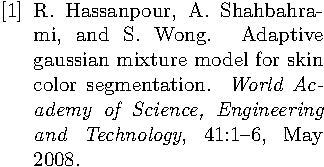
\includegraphics[width=0.45\textwidth,%
							   trim=0 -14 0 0]{\latexbokFiguredir/5/abbrv.pdf}}
	} \hfil % (end)
	\subfloat[\texttt{alpha.bst}]{% (fold)
		\fbox{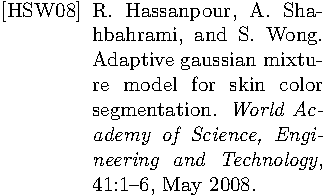
\includegraphics[width=0.45\textwidth]{\latexbokFiguredir/5/alpha.pdf}}
	} \\ % (end)
	\subfloat[\texttt{apalike.bst}]{\label{fig:bibstyle:apalike}% (fold)
		\fbox{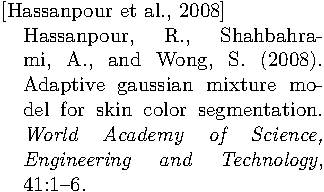
\includegraphics[width=0.45\textwidth]{\latexbokFiguredir/5/apalike.pdf}}
	} \hfil % (end)
	\subfloat[\texttt{chscite.bst} från \pack{chscite}]{% (fold)
		\label{fig:bibstyle:chscite}%
		\fbox{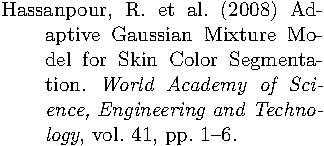
\includegraphics[width=0.45\textwidth,%
							   trim=0 -22 0 0]{\latexbokFiguredir/5/chscite.pdf}}
	} \\ % (end)
	\subfloat[\texttt{dcu.bst} från \pack{harvard}]{% (fold)
		\fbox{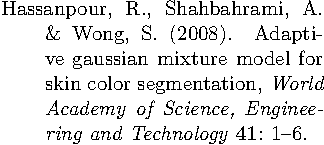
\includegraphics[width=0.45\textwidth,%
							   trim=0 -11.5 0 0]{\latexbokFiguredir/5/harvard-dcu.pdf}}
	} \hfil % (end)
	\subfloat[\texttt{jurabib.bst} från \pack{jurabib}]{% (fold)
		\label{fig:bibstyle:jurabib}%
		\fbox{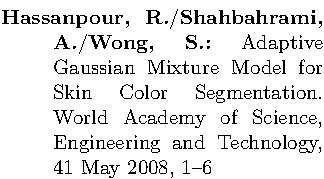
\includegraphics[width=0.45\textwidth,%
							   trim=0 0 0 5,clip=true]{\latexbokFiguredir
							   /5/jurabib.pdf}}
	} \\ % (end)
	\caption[Några av de bibliografistilar som kan åstadkommas med
	hjälp av \BibTeX.]{Några av de bibliografistilar som kan åstadkommas
	med hjälp av \BibTeX.
	Figurerna~\subref{fig:bibstyle:abbrv}–\subref{fig:bibstyle:apalike} 
	visar standardstilar, medan  
	figurerna~\subref{fig:bibstyle:chscite}–\subref{fig:bibstyle:jurabib} 
	visar stilar som definieras av olika paket.}
	\label{fig:bibstyle}
\end{figure}

\subsubsubsection*{Harvard- och Chicago-stilen: \pack{harvard} och \pack{chscite}}\label{sec:5:harvard}
Harvard- och Chicago-stilarna, varav den senare beskrivs utförligt i
\emph{The Chicago Manual of Style} \parencite{Chicago10},
är sätt att referera till källor baserat
på deras författare, och används ofta i de humanistiska vetenskaperna.
Fördelen med dessa stilar är att referenserna smälter in bättre med den
omgivande texten och ger ett bättre sammanhang.

Tyvärr så är \BibTeX{} från början inte gjort för att stödja de här
referensstilarna, varför det har dykt upp ett antal olika paket som
gör det möjligt. Ett av dessa paket är \pack{harvard}, som beskrivs
utförligt av \textcite{Williams08}. Paketet definierar förutom det
vanliga kommandot \cmd{cite} tre relativt självförklarande kommandon:
\cmd{citeasnoun}, som refererar till en källa som ett substantiv,
\cmd{possessivecite}, som refererar till en källa i genitivform,
och \cmd{citeaffixed}, som refererar som \cmd{cite} men med ett tillägg.
Hur dessa bör användas i text illustreras av följande exempel:
\begin{latexcode}
...vilket visades av \citeasnoun{Hassanpour08}.
\possessivecite{Hassanpour08} undersökning visade att...
...flera rapporter \citeaffixed{Hassanpour08}{t.ex.}...
\end{latexcode}
	
\label{sec:chscite}
Chalmers rekommenderar att man använder en stil baserad på Chicago-%
stilen \parencite{ChsLib10}, och dessa rekommendationer implementeras av 
paketet \pack{chscite} som bygger på \pack{harvard} och därför fungerar
på samma sätt. Även detta paket finns på CTAN.
\end{document}
